\documentclass{article}
\usepackage[ngerman]{babel}
\usepackage{graphicx}
\usepackage{subcaption}
\usepackage{acro}
\usepackage{pdfpages}

\title{Echtzeitfähige Deep-Learning-basierte Spurerkennung}
\author{Tim Alkofer, Jan-Marcel Schmidt}
\date{Oktober 2024} %Todo

\begin{document}
    \pagenumbering{Roman}
    
    \maketitle
    
    \begin{tabbing}
    \hspace{5em} \= \\
        Zeitraum: \> 04.2024-10.2024 \\ %Todo
        Hochschule: \> HTWG Konstanz \\
        Rahmen: \> Teamprojekt Autombilinformationstechnik \\
        Betreuer: \> Prof. Dr. Christopher Knievel \\
        Abgabe: \> 26.03.2024 \\ %Todo
    \end{tabbing}

    \clearpage
    \tableofcontents
    \clearpage
    \listoffigures
    \clearpage
    \bibliographystyle{plain}
    \bibliography{literatur}
    % \clearpage
    % \printacronyms
    \clearpage
    \pagenumbering{arabic}

    \section{Einleitung}
        Im Rahmen des Studiums Automobilinformationstechnik an der HTWG Konstanz wird im sechsten Semester ein Teamprojekt durchgeführt.
        Im folgenden soll das Projekt \textit{Echtzeitfähige Deep-Learning-basierte Spurerkennung} vorgestellt werden.

        \subsection{Ausgangssituation}
            % Auto beschrieben
            Das \textit{HTWG-RaceCar} ist ein autonomes Modellfahrzeug, welches im Rahmen des Studiums Automobilinformationstechnik an der HTWG Konstanz entwickelt wird.
            Das Fahrzeug ist mit einem NVIDIA Jetson Orin Nano Developer Kit
            ausgestattet, welcher die Steuerung des Fahrzeugs übernimmt.
            Dabei kann das Fahrzeug sowohl im manuellen Modus per Tastatur gesteuert, als auch im autonomen Modus betrieben werden.
            Zur Erkennung der Spur wird eine Kamera verwendet. %Todo Kamera-Name
            In der vorherigen Umsetzung wurde eine Kantendetektion verwendet, um die Spurmarkierungen zu erkennen.
            Mit Hilfe der Python-Bibliothek OpenCV wurden die Kanten der Spurmarkierungen wie folgt erkannt:
            Zunächst wurde das aufgenommene Farbbild mit der Methode \textit{cv2.cvtColor()} in Graustufen konvertiert, um anschließend mit \textit{cv2.GaussianBlur()} eine gaußsche Weichzeichnung durchzuführen, die das Ziel hatte Rauschen zu reduzieren und Details zu glätten. Im Anschluss sollten mit \textit{cv2.Canny()} Kanten identifiziert werden. Diese Methode arbeitet mit Ableitungen und nimmt an, dass Bereiche mit starken Änderungen Kanten entsprechen.
            Aus diesen Kanten wurden mit \textit{cv2.HoughLinesP()} Linien errechnet. 
            Die Probleme dieses Systems waren hohe Anfälligkeit gegenüber Lichtverhältnissen in Form von Spiegelungen und Schatten.
            Eine autonome Navigation des Fahrzeugs war somit nur unter optimalen Bedingungen möglich. Diese bestanden in zugezogenen Vorhängen im Labor.
            Doch selbst unter diesen Bedingungen war die Erkennung der Spurmarkierungen nicht immer zuverlässig.

            Eine Deep-Learning-basierte Spurerkennung soll diese Probleme beheben und eine zuverlässige Spurerkennung auch unter schwierigen Bedingungen ermöglichen.

 
            % Todo am besten quantifizieren

        \subsection{Aufgabenstellung}
            % siehe OneNote
            \textit{In dem Teamprojekt ist ein neuronales Netzwerk zu implementieren, das in der Lage ist, Spurmarkierungen robust zu erkennen. Dieses Netzwerk soll in weniger als 60 Millisekunden eine Vorhersage der Spurmarkierungen auf dem Jetson Nano liefern.}
            % 
    \section{Umsetzung}
        % Als grundlage diente repository x/y
        Um den Umfang des Projekts zu begrenzen, wurde das bestehendee Repository \textit{lanedet} als Grundlage verwendet.
        %Todo: Link einfügen: https://github.com/Turoad/lanedet
        \textit{LaneDet is an open source lane detection toolbox based on PyTorch that aims to pull together a wide variety of state-of-the-art lane detection models.}

        %\subsection{Recherche}
            % 
        \subsection{Installation}
            Das erste Ziel der Umsetzung bestand darin das besagte Repository auf den WorkingStations des KI-Labors zu installieren, um selbst Modelle trainieren zu können.
            Anfängliche Probleme von Paketabhängigkeiten und Versionskonflikten konnten aufgelöst werden. 
            %Todo: landeDet auf HTWG Git schieben
            % ToDo: genaue Versionen pyTorch/cuda etc
            Alle Änderungen können in der GIT-History nachvollzogen werden und über ergänzte Installationsskripte reproduziert werden, sodass das Projekt auch nach Abschluss des Teamprojekts weitergeführt werden kann. Letzter Stand: 15.01.2025. %Todo: Datum
            Zur Installation auf WorkingStations und Jetson können die Skripte \textit{scripts\textbackslash install\_workstation.sh} und \textit{scripts\textbackslash install\_jetson.sh} wie in der \textit{Read.me} beschrieben verwendet werden.

        \subsection{Aufbau neuronales Netz}
            Das verwendete Repository lane bietet eine Reihe von verschiedenen Architekturen, Backbones und Datensätzen, die für die Spurerkennung verwendet werden können.
            Um möglichst schnell einen Überblick über die verschiedenen Möglichkeiten zu bekommen, wurden zunächst die vorgegebenen Modelle trainiert und subjektiv getestet.
            Dabei wurde berücksichtigt ob und wie gut die verschiedenen Modelle die Spurmarkierungen ahand von Beispielbildern aus dem Labor erkennen konnten.
            % Todo: Bilder einfügen

            \subsubsection{Datengrundlage}
            % --> auswahl aufgrund von bester subjektiver performance
            % nachweise für daten
            Als Datengrundlage verlinkt LaneDet auf CULane oder alternativ TUSimple, die beide bereits annotierte Datensätze für die Spurerkennung bereitstellen. 
            %Todo: Links einfügen
            % ToDo: Beschreiben wie entpackt werden muss
                Nach einer subjektiven Bewertung der Datensätze wurde sich zunächst für TUSimple entschieden, da dieser eine bessere Performance aufwies.
            %Todo Bilder einfügen
            Während erster Tests ist klar geworden, dass die Bildauflösung eine entscheidende Rolle für die Erkennung spielt. Anfangs wurde im besten Bild die unterschiedliche Farbe der Spurmarkierungen vermutet. Diese konnte jedoch durch nachbearbeitung der Bilder ausgeschlossen werden.

            \subsubsection{Backbone}
            Wie bei der Datengrundlage stellt LaneDet auch eine Liste an Backbones zur Verfügung. Auch hier wurde zunächst subjektv entschieden, welcher Backbone die beste Erkennung liefert.
            Auf dem Labor-PC konnten dabei mit dem Mobile-Net Backbone die besten Ergebnisse erzielt werden.
            %Todo: Bilder einfügen
            %Todo: Graphen einfügen
            \subsubsection{Architekturen}
                Für die verschiedenen Architekturen standen im lanedet-Repository verschiedene Konfigurationen zur Verfügung, die nachfolgend kurz zusammengefasst werden.

                \textbf{Condlane} (\textit{Conditional Lane Detection}) ist eine Architektur, die sich auf die Erkennung von Fahrspuren mit komplexen Topologien, wie z.B. dichte, gekrümmte und verzweigte Linien spezialisiert hat. Diese Architektur nutzt Conditional-Shape-Decoder-Konzept, bei dem die Spur als ein diskretes Set von Punkten repräsentiert wird. Die Spurerkennung wird durch konditionierte Dekodierung basierend auf einem Feature-Extraktionsprozess ermöglicht. Die Stärken von Condlane liegen in der robusten Erkennung von Fahrspuren selbst in komplexen Szenarien wie starken Okklusionen und dichten Linien.
                \cite{Ganeriwala2023Cross}

                \textbf{LaneATT} (\textit{Lane Attention Network}) ist eine Architektur, die sich auf die Effizienz und Genauigkeit der Fahrspurerkennung konzentriert. Sie verwendet einen Aufmerksamkeitsmechanismus, um wichtige Merkmale zu verstärken und die globale Kontextinformation zu erfassen. Der Anwendungsbereich liegt vor allem in strukturierten Umgebungen, bei denen eine hohe Genauigkeit gefordert ist. 
                \cite{He2021Fast}

                \textbf{RESA} (\textit{Recurrent Feature-Shift Aggregator}) ist eine Architektur, die darauf abzielt, Fahrspuren in komplexen Szenarien präzise zu erkennen. Sie nutzt eine rekurrente Verschiebung von Merkmalen, um die räumlichen Beziehungen von Pixeln zu erfassen und globale Informationen zu sammeln. RESA kombiniert grob- und feindetaillierte Merkmale in der Hochskalierungsphase, um eine pixelgenaue Vorhersage zu ermöglichen.
                \cite{Zheng2020RESA}

                \textbf{SCNN} (\textit{Spatial-Temporal Convolutional Neural Network}) ist eine Architektur, die räumlich-zeitliche Informationen nutzt, um die Erkennung von Fahrspuren zu verbessern. Sie verwendet ein Encoder-Decoder-Framework und integriert räumlich-zeitliche rekurrente Module, um zusammenhängende Informationen aus Bildsequenzen zu extrahieren. SCNN zeigt eine hohe Genauigkeit und Effizienz in Echtzeitszenarien.
                \cite{Li2024Enhanced}

                \textbf{UFLD} (\textit{Ultra Fast Lane Detection}) ist eine Architektur, die auf Geschwindigkeit und Effizienz optimiert ist. Sie verwendet eine Bottom-Up-Strategie, um Fahrspuren schnell zu erkennen, und zeigt eine hohe Leistung auf gängigen Datensätzen wie CULane und TuSimple. UFLD ist bekannt für seine Fähigkeit, schnell und mit hoher Genauigkeit zu arbeiten.
                \cite{Xu2024Exploring}

            \subsubsection{Konfigurationsauswahl}
                Nach subjektiver Bewertung der verschiedenen Modelle wurde sich für das Modell mit dem Mobile-Net Backbone und der Architektur laneatt in Kombination mit dem TUSimple Datensatz entschieden, da dort zunächst die besten Spurerkennungen erzielt werden konnten.
                In späteren Tests konnten die zunächst subjektiv ausgewählten Kriterien auch mit Zahlen belegt werden, wie Abbildung \ref{fig:Modell_Auswertung} zeigt.
                Die spalte BestMetric ist dabei mit dem F1-Score gleichzusetzen, der während der Validierung der Modelle berechnet wird.
                %Todo: F1-Score erklären?
                \begin{figure}[h!]
                    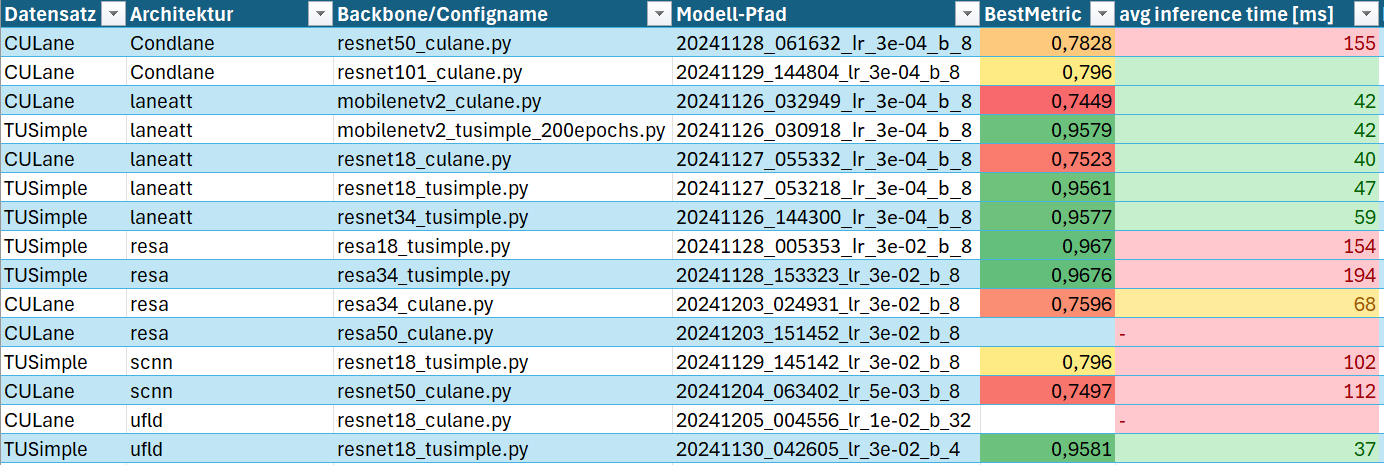
\includegraphics[width=\linewidth]{Auswertung_BackBone_Datensatz.png}
                    \caption{Modell-Auswertung}
                    \label{fig:Modell_Auswertung}
                \end{figure}
                Wie die Grafik aufzeigt, ist der TUSimple-Datensatz mit einem F1-Score von etwa 0.95 dem CULane-Datensatz mit einem Wert von etwa 0.75 deutlich überlegen.

        \subsection{Performance}
            % --> performance der modelle auf Labor PC's
            % --> performance der Modelle auf altem Jetson

            % Todo Performance in Bildern/Excel zeigen
            
            Erste Tests auf dem Jetson Nano zeigten jedoch, dass die Modelle nicht in Echtzeit betrieben werden konnten. Eine verarbeitszeit von etwa 20 Sekunden pro Bild war zu langsam.
            Um dieses Problem zu lösen wurde versucht das Modell zu quantisieren, was jedoch nicht zum Erfolg führte.
            Eine Konvertierung in das ONNX-Format, konnte zwar durchgeführt werden, jedoch wurden keine Linien mit der konvertierten Variante erkannt.
            %Todo mehr ausführen @Mars?
            Nach anschaffung eines neuen Jetson Nano konnte die Performance des Modells auf dem Jetson Nano deutlich verbessert werden, sodass keine weitere Anpassung mehr nötig waren.
            %Todo: Performance auf neuem Jetson einfügen was für zeiten haben wir hier?
        \subsection{Steuerung}
            % alte Steuerung
            % Projekt während Autonomes Fahren
            % neue Steuerung
    \section{Fazit}
        % Ergebnisse
        % Vgl alte Spurerkennung vs neue Spurerkennung --> Bild
        % Probleme
        % Ausblick


\end{document}